\documentclass[../main.tex]{subfiles}
\begin{document}
	\chapter{Neural Networks} \label{ch:neural}

\noindent \textit{Neural Networks} are the quintessential deep learning models, especially \textit{multilayer feedforward networks}.  A single layer of a deep learning model, also called an\textit{ artificial neuron}. They are widely used for nonlinear function approximation. The goal of a deep neural network is to approximate some function $f^*$. For example, for a classifier, $y = f^*(x)$ maps an input $x$ to a category $y$.  \\ \\ 
%A feedforward network defines a mapping $y = f(x;\theta)$ and learns the value of the parameters $\theta$ that result in the best function approximation. \\ \\ 
\noindent The term \textit{neural} refers  to the fact that this model was originally inspired by how biological neurons process information. These artificial neurons mimic the processing of information in biological neurons. \\ \\ 
\noindent The term \textit{feedforward} indicates the direction of information flow within the network, moving only forward in contraposition to backwards. Each layer processes the input data and passes its output to the next layer, creating a sequence of transformations until the final output is produced. $f(f_1(f_2(f_3)))$ \\ \\
\noindent The term \textit{network} refers to the interconnected structure of artificial neurons. An multilayer network consists of multiple layers, including an input layer, one or more hidden layers, and an output layer. \\ \\ %The neurons within each layer are connected to the neurons in the subsequent layer, forming a network of connections. The connections between neurons are represented by weights, which determine the strength and influence of each neuron's output on the inputs of the subsequent layer. \\ \\ 
\noindent The architecture of the network entails determining its \textit{depth}, \textit{width}, and \textit{activation functions} used. Depth is the number of hidden layers. Width is the number of units (nodes) on each hidden layer. 

\begin{figure}[h]
	\centering
	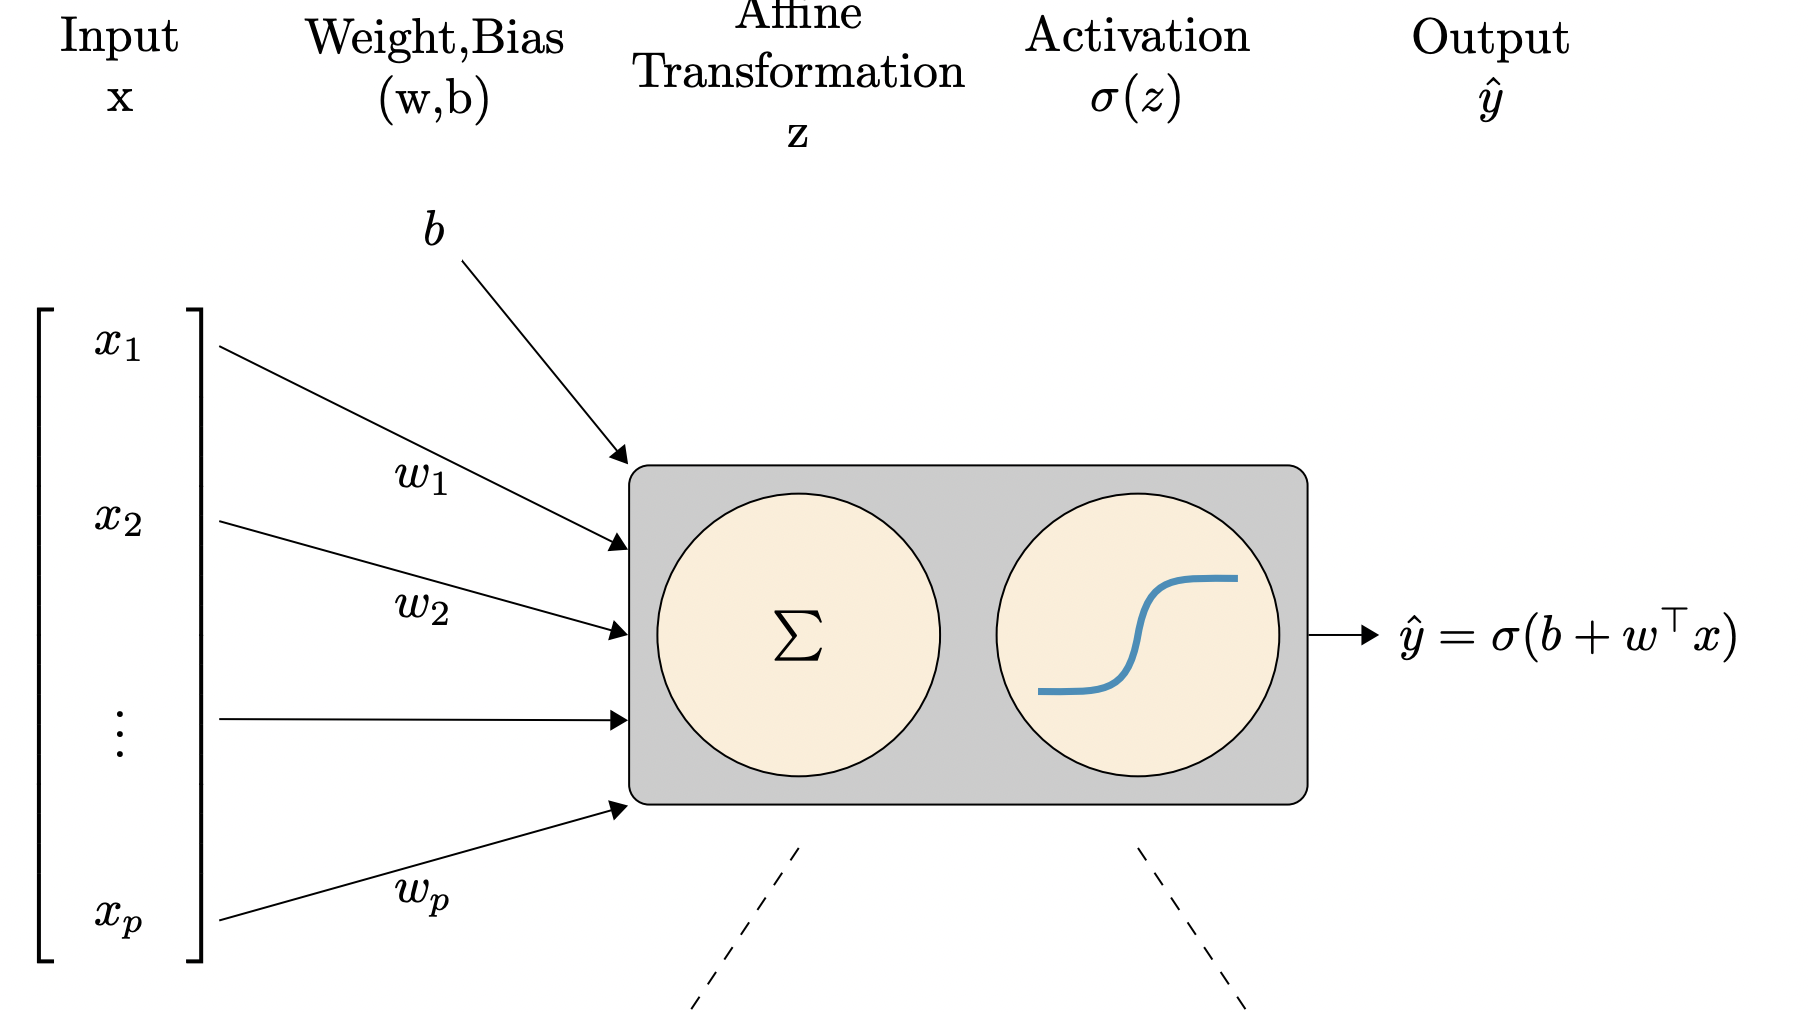
\includegraphics[width=0.6\linewidth]{imgs/neu}
\end{figure} \mbox{} \par
	
	
	%they are composed of interconnected processing units called artificial neurons, which are organized in layers and are capable of learning and generalizing from data.	
	\section{Architecture of a Multilayer Feedforward Network}

	\noindent A single layer of a deep learning model, also called an\textit{ artificial neuron }is represented by $$ y=\sigma(w^Tx + \theta) $$
Observe that the artificial neuron is composed of an affine transformation $ z=w^Tx + \theta$ followed by a (generally) non-linear transformation $\sigma(z)$. \\ \\ 
		\noindent  We now get into more details on the precise definition of a deep neural network, which is after all a purely mathematical object. 
	\begin{definition} A \textit{multilayer feedforward network} is the function
		$$f(x)=\sum_{j=1}^k \beta_j \cdot \sigma(w_j \cdot x - \theta_j)$$
		where $x \in \mathbb{R}^n$ is the input vector, $k \in \mathbb{N}$ is the number of processing units in the hidden layer, $w_j \in \mathbb{R}^n$ is the weight vector that connects the input to processing unit $j$ in the hidden layer, $\sigma : \mathbb{R} \rightarrow \mathbb{R}$ is an activation function, $\theta_j \in \mathbb{R}$ is the threshold (or bias) associated with processing unit $j$ in the hidden layer, and $\beta_j \in \mathbb{R}$ is the weight that connects processing unit $j$ in the hidden layer to the output of the network.
		
		
	\end{definition}

	\noindent Let $N_{w}$ be the family of all functions implied by the network's architecture.  If we can show that $N_{w}$ is dense in $C(\mathbb{R}^n)$, we can conclude that for every continuous function $g \in C(\mathbb{R}^n) $ and each compact set $K \subset \mathbb{R}^n$, there is a function $f \in N_{w}$ such that $f$ is a good approximation to $g$ on K. \\ \\
	\noindent Under which necessary and sufficient conditions on $\sigma$ will the family of networks $N_w$ be capable of approximating to any desired accuracy any given continuous function?
	
	
\end{document}